% Pre-ambulo
\documentclass[a4paper, 12pt]{abnt}

\usepackage[brazil]{babel}
%\usepackage[latin1]{inputenc}
\usepackage[utf8]{inputenc}
\usepackage[T1]{fontenc}
\usepackage{dsfont}
\usepackage{amssymb,amsmath}
\usepackage{multirow}
\usepackage[alf]{abntcite}
\usepackage[pdftex]{color, graphicx}
\usepackage{colortbl}
\usepackage{url}
\usepackage{abnt-alf}
\usepackage{abntcite}
\usepackage{algorithm}
\usepackage{algorithmic}
\usepackage{graphicx}
\usepackage{subcaption}
%\usepackage{minted} 
%\usepackage{alg}
%\usepackage{hyperref}
\usepackage{soul}

% Redefinicao de instrucoes
\floatname{algorithm}{Algoritmo}
\renewcommand{\algorithmicrequire}{\textbf{Entrada:}}
\renewcommand{\algorithmicensure}{\textbf{Saída:}}
\renewcommand{\algorithmicend}{\textbf{fim}}
\renewcommand{\algorithmicif}{\textbf{se}}
\renewcommand{\algorithmicthen}{\textbf{então}}
\renewcommand{\algorithmicelse}{\textbf{senão}}
\renewcommand{\algorithmicfor}{\textbf{para}}
\renewcommand{\algorithmicforall}{\textbf{para todo}}
\renewcommand{\algorithmicdo}{\textbf{faça}}
\renewcommand{\algorithmicwhile}{\textbf{enquanto}}
\renewcommand{\algorithmicloop}{\textbf{loop}}
\renewcommand{\algorithmicrepeat}{\textbf{repetir}}
\renewcommand{\algorithmicuntil}{\textbf{até que}}
\renewcommand{\algorithmiccomment}[1]{\% #1}


% Definicao da lista de simbolos
% \simb[entrada na lista de simbolos]{simbolo}:
% Escreve o simbolo no texto e uma entrada na lista de simbolos.
% Se o parametro opcional e omitido, usa-se o parametro obrigatorio.
\newcommand{\simb}[2][]
{%
	\ifthenelse{\equal{#1}{}}
	{\addcontentsline{los}{simbolo}{#2}}
	{\addcontentsline{los}{simbolo}{#1}}#2
}
% Para aceitar comandos com @ (at) no nome
\makeatletter 
% \listadesimbolos: comando que imprime a lista de simbolos
\newcommand{\listadesimbolos}
{
	\pretextualchapter{Lista de símbolos}
	{\setlength{\parindent}{0cm}
	\@starttoc{los}}
}
% Como a entrada sera impressa
\newcommand\l@simbolo[2]{\par #1}
\makeatother


% Definicao da lista de abreviaturas e siglas
% \abrv[entrada na lista de simbolos]{abreviatura}:
% Escreve a sigla/abreviatura no texto e uma entrada na lista de abreviaturas e siglas.
% Se o parametro opcional e omitido, usa-se o parametro obrigatorio.
\newcommand{\abrv}[2][]
{%
	\ifthenelse{\equal{#1}{}}
	{\addcontentsline{loab}{abreviatura}{#2}}
	{\addcontentsline{loab}{abreviatura}{#1}}#2
}
% Para aceitar comandos com @ (at) no nome
\makeatletter 
% \listadeabreviaturas: comando que imprime a lista de abreviaturas e siglas
\newcommand{\listadeabreviaturas}
{
	\pretextualchapter{Lista de abreviaturas e siglas}
	{\setlength{\parindent}{0cm}
	\@starttoc{loab}}
}
% Como a entrada sera impressa
\newcommand\l@abreviatura[2]{\par #1}
\makeatother


% \listofalgorithms: comando que imprime a lista de algoritmos
\renewcommand{\listalgorithmname}{Lista de algoritmos}

\newcommand*\rot{\rotatebox{90}}

% Hifenização de palavras feita de forma incorreta pelo LaTeX
\hyphenation{PYTHON ou-tros}


% Inicio do documento
\begin{document}

	\frenchspacing
	
	% Capa (arquivo Includes/Capa.tex)
	% Capa
% Proteção externa do trabalho e sobre a qual se imprimem as informações indispensáveis 
% à sua identificação.

% Especificação da capa
\begin{titlepage}
	\begin{center}
		
		% Cabeçalho (não deve ser modificado)
		% Contém o brasão da Universidade, o logotipo do Departamento, além dos dados
		% relacionados à vinculação do aluno (Universidade, Centro, Departamento e Curso)
		\begin{minipage}{2cm}
			\begin{center}
				\includegraphics[width=1.7cm, height=2.0cm]{Imagens/Brasao-UFRN.jpg}
			\end{center}
		\end{minipage}
		\begin{minipage}{11cm}
			\begin{center}
				\begin{espacosimples}
					{\small \textsc{Universidade Federal do Rio Grande do Norte}			\\
							  \textsc{Centro de Tecnologia}						\\
							  \textsc{Departamento de Engenharia de Computação e Automação}	\\
							  \textsc{Bacharelado em Engenharia de Computação}}
				\end{espacosimples}
			\end{center}
		\end{minipage}
		\begin{minipage}{2cm}
			\begin{center}
				\includegraphics[width=1.8cm, height=1.5cm]{Imagens/Logotipo-DCA.jpg}
			\end{center}
		\end{minipage}
			
		\vspace{6cm}
						
		% Título do trabalho
		{\setlength{\baselineskip}%
		{1.3\baselineskip}
		{\LARGE \textbf{Configurações otimizadas de energia para aplicações em computação de alto desempenho}}\par}
			
		\vspace{4cm}
			
		% Nome do aluno (autor)
		{\large \textbf{Vitor Ramos Gomes da Silva}}
						
		\vspace{7cm}
		
		% Local da instituição onde o trabalho deve ser apresentado e ano de entrega do mesmo
		Natal-RN\\ \today%03 de maio de 2018
	\end{center}
\end{titlepage}

	% Folha de rosto (arquivo Includes/FolhaRosto.tex)
	% Folha de rosto
% Contém os elementos essenciais à identificação do trabalho.

% Título, nome do aluno e respectivo orientador e filiação
\titulo{\Large{Configurações otimizadas de energia para aplicações em computação de alto desempenho}}
\autor{Vitor Ramos Gomes da Silva}
\orientador[Orientador]{\par Prof. Dr. Samuel Xavier de Souza}
\coorientador[Co-Orientador]{\par Prof. Dr. Alex Furtunato}

\instituicao
{
	Universidade Federal do Rio Grande do Norte -- UFRN \par 
	Departamento de Engenharia de Computação e Automação -- DCA
}
	
% Natureza do trabalho (não deve ser modificada)
\comentario
{
Trabalho de Conclusão de Curso apresentado ao Departamento de Engenharia de Computação e Automação do Centro de Tecnologia da Universidade Federal do Rio Grande do Norte como parte dos requisitos necessários para obtenção do grau de Engenheiro de Computação com habilitação em Automação Industrial.
}
		
% Local e data
\local{Natal-RN}
\data{\today}
	
\folhaderosto	
	
	% Folha de aprovacao (arquivo Includes/FolhaAprovacao.tex)
	% Folha de aprovação
\begin{folhadeaprovacao}
	\setlength{\ABNTsignthickness}{0.4pt}
	\setlength{\ABNTsignwidth}{10cm}
	
	% Informações gerais acerca do trabalho 
	% (nome do autor, título, instituição à qual é submetido e natureza)
	\noindent 
	Monografia de Graduação sob o título \textit{Configurações otimizadas de energia para aplicações em computação de alto desempenho} apresentada por 
	Vitor Ramos Gomes da Silva e aceita pelo Departamento de Engenharia de Computação e Automação do
	Centro de Tecnologia da Universidade Federal do Rio Grande do Norte,
	sendo aprovada por todos os membros da banca examinadora abaixo especificada:
		
	% Membros da banca examinadora e respectivas filiações
	\assinatura
	{
		Prof. Dr. Samuel Xavier de Souza\\
		{\small Orientador(a)} 															\\ 
		{\footnotesize
			Departamento de computação e automação																	\\
		  	Universidade Federal do Rio Grande do Norte
		}
	}
	
	\assinatura
	{
		Prof. Dr. Alex Furtunato							
		\\
		{\small Co-orientador(a)}							
		\\ 
		{\footnotesize
			Departamento 																	\\
		  	O Instituto Federal de Educação, Ciência e Tecnologia do Rio Grande do Norte
		}
	}
		
	\assinatura
	{
		Luiz Felipe de Queiroz Silveira 						 \\ 
		{\footnotesize
			Departamento de computação e automação 																	 \\
		  	Universidade Federal do Rio Grande do Norte
		}
	}
		
% 	\assinatura
% 	{
% 		Titulação e nome do membro da banca examinadora 						 \\ 
% 		{\footnotesize
% 			Departamento 																	 \\
% 		  	Universidade
% 		}
% 	}
		
	\vfill
	
	\begin{center}
		Natal-RN, \today.
	\end{center}
\end{folhadeaprovacao}	
	
	% Dedicatoria (arquivo Includes/Dedicatoria.tex)
	% Dedicatória

\chapter*{}
\vspace*{\fill}
\begin{text}
\centering
\noindent
\textit{Aos meus pais e irmão que, com muito carinho e apoio, não mediram esforços para que eu chegasse até esta etapa tão importante em minha vida. Não posso esquecer dos meus amigos e colegas, pelo incentivo e pelo apoio constantes. E a todos aqueles que de alguma forma contribuíram no meu caminhar pelas pedras até esse momento.}
\end{text}
\vspace*{\fill}

% \vspace{15cm}
% \begin{flushright}
% Aos meus pais, que com muito carinho e apoio não mediram esforços para que eu chegasse até a esta etapa da minha vida.
% \end{flushright}
	
	% Agradecimentos (arquivo Includes/Agradecimentos.tex)
	% Agradecimentos

\chapter*{Agradecimentos}
Aos meus pais, Cláudia Ramos Gomes da Silva e Paulo Sérgio Gomes da Silva, por tudo. A minha irmã, meus primos e amigos especialmente Andressa Stefany pelo apoio. Aos meus orientadores Samuel Xavier de Souza, que propôs a ideia para este trabalho e Alex Furtunato que co-orientou. A todos os professores do curso de Engenharia de Computação, que sempre estiveram dispostos a ajudar e contribuir para um melhor aprendizado. Ao NPAD e aos servidores Pedro Klisley e Daniel Holanda por também colaborarem na pesquisa. E a todos que direta ou indiretamente fizeram parte da minha formação, obrigado.
   
   % Epigrafe (arquivo Includes/Epigrafe.tex)
	% Epígrafe (citação seguida de indicação de autoria)

\chapter*{}
\vspace{15cm}
\begin{flushright}
	\textit
	{
		``Na vida, não existe nada a temer, mas a entender.``
	}\medskip\\ 
	(Marie Curie)
\end{flushright}
	
	% Resumo em língua vernacula (arquivo Includes/Resumo.tex)
	% Resumo em língua vernácula
\begin{center}
	{\Large{\textbf{Configurações otimizadas de energia para aplicações em computação de alto desempenho}}}
\end{center}

\vspace{1cm}

\begin{flushright}
	Autor: Vitor Ramos Gomes da Silva\
	Orientador: Prof. Dr. Samuel Xavier de Souza
\end{flushright}

\vspace{1cm}

\begin{center}
	\Large{\textsc{\textbf{Resumo}}}
\end{center}

\noindent 
Este trabalho propõe uma metodologia para minimizar o consumo de energia 
em computação de alta performance, encontrando os parâmetros ideais de frequência e núcleos ativos no processador. A partir de uma modelagem da potência do sistema, desenvolvida com base no consumo de potência do circuito CMOS e uma estimativa do tempo de execução da aplicação utilizando inteligência artificial, é calculada a equação da energia em função da frequência, número de núcleos e entrada da aplicação. Com esta equação, é encontrada a configuração que minimiza o consumo total de energia. Foram feitos testes em quatro aplicações e os resultados desse método mostraram que essa abordagem chegou à economia de até 30\% quando comparado ao esquema de economia de energia existente atualmente no Linux.


\noindent\textit{Palavras-chave}: Software energeticamente eficiente, Modelagem do consumo de potência, Escalonamento de frequência
	
	% Abstract, resumo em língua estrangeira (arquivo Include/Abstract.tex)
	% Resumo em língua estrangeira (em inglês Abstract, em espanhol Resumen, em francês Résumé)
\begin{center}
	{\Large{\textbf{Energy-Optimal Configurations for high performance computer applications}}}
\end{center}

\vspace{1cm}

\begin{flushright}
	Author: Vitor Ramos Gomes da Silva\\
	Advisor: Prof. Dr. Samuel Xavier de Souza
\end{flushright}

\vspace{1cm}

\begin{center}
	\Large{\textsc{\textbf{Abstract}}}
\end{center}

\noindent This work proposes a methodology to minimize energy consumption
in high-performance computing by finding the ideal frequency and active cores parameters in the processor. Based on a model of the power draw of the system, developed based on the power consumption of the CMOS circuit, and an estimation of the execution time of the application using artificial intelligence is calculated the energy equation with frequency, number of active cores and input of the application as variables and from this equation is found the configuration that minimizes the total power consumption. The results of this method in four applications show that the proposed approach achieved savings of more than 30 \% when compared to the current energy saving scheme in Linux.

\noindent\textit{Keywords}: 
Energy Efficient Software, Energy Modeling, Frequency Scaling.
	
	% Lista de figuras
	\listoffigures

	% Lista de tabelas
	\listoftables
	
	% Lista de abreviaturas e siglas
	\listadeabreviaturas
	
	% Lista de símbolos
	%\listadesimbolos
	
	% Lista de algoritmos (se houver)
	% Devem ser incluídos os pacotes algorithm e algorithmic
	% \listofalgorithms
	
	% Sumário
	\sumario
	
	
	% Parte central do trabalho, englobando os capítulos que constituem o mesmo
	% Os referidos capítulos devem ser organizados dentro do diretório "Capítulos"
	
	%\pagenumbering{arabic}
    \setcounter{page}{1}
	
	% Capitulo 1: Introdução (arquivo Includes/Introducao.tex)
	% Introdução
\chapter{Introdução} \label{cap:introducao}

Consumo de energia é uma preocupação na computação moderna, tanto em dispositivos pessoais, smartphones e notebooks, visando economia da bateria do dispositivo, como em grandes servidores, nuvens e sistemas computacionais de alto desempenho devido aos custos de manutenção e impacto ambiental que eles podem gerar.

Em computação de alto desempenho \abrv[HPC --High Performance Computing]{(HPC)} isso é mais complicado, pois, facilmente um sistema chega a consumir centenas de KiloWatts e sistemas com maior poder computacional podem chegar até a dezenas de MegaWatts \cite{Top500}. Isso pode inviabilizar projetos ou até mesmo descontinuar trabalhos existentes por falta de recursos. Além disso, a próxima geração de sistemas HPC com capacidade de processamento de exaFLOPS, isto é, bilhões de bilhões de cálculos por segundo, terão seu uso restrito pelo seu consumo de energia \cite{Alfonso2013}.

Investir em novas maneiras de reduzir o consumo de potência é crucial para esses sistemas se tornarem viáveis economicamente, além da redução do impacto ambiental causado pelo alto consumo deles. Há muitas pesquisas nesta área, e portanto, diversas formas de reduzir o consumo de energia. Uma das principais é através do consumo de energia do processador. Pesquisas do Google \cite{Fan2007} mostraram que ele é o principal componente responsável pelo consumo de energia em servidores, chegando no pico a 57\% da energia total gasta pelo sistema \cite{Barroso2007}.

Por isso, processadores atuais incluem diversos componentes para minimizar a potência utilizada, como, unidades independentes que podem ser desabilitadas \cite{Rotem2012}, clock gating: técnica utilizada em circuitos síncronos para diminuir o consumo de energia \cite{Srinivasan2015}, Dynamic Voltage and Frequency Scaling \cite{Mittal2014} \abrv[DVFS -- Dynamic Voltage and Frequency Scaling]{(DVFS)}, entre outras.

A técnica de DVFS \cite{Hackenberg2015, Dzhagaryan2014, Hahnel2012, Basmadjian2012, Travers2015, Miyoshi2002, Anghel2011, Pietri2014, Spiga2006} é umas das mais eficientes, pois, o consumo do processador está altamente correlacionado com a sua frequência de operação. Esta consiste em controlar a frequência e a voltagem de acordo com a utilização do dispositivo. Este controle pode ser feito tanto em software através do sistema operacional, quanto em hardware.

Este trabalho propõe uma metodologia para encontrar a frequência operacional e o número de núcleos ativos que minimizam a energia total usada para executar uma aplicação HPC em um único nó com memória compartilhada. Essa metodologia é diferente dos existentes no Linux, pois utiliza uma modelagem do consumo de potência junto com uma caracterização do tempo de execução da aplicação para melhor encontrar a configuração que minimiza a energia total utilizada.

O modelo de potência baseia-se na modelagem da potência do circuito lógico CMOS em função da frequência de operação \cite{Sarwar1997}, incluindo a potência dinâmica, estática e de fuga. Além da frequência de operação, o modelo de energia também é parametrizado para o número de soquetes ativos e de núcleos ativos por soquete.

A modelagem do desempenho é feita pela caracterização da aplicação na arquitetura de destino. A ideia é prever o desempenho da aplicação em qualquer configuração específica. O modelo utiliza a frequência de operação, o número de núcleos ativos e o tamanho da entrada. Essa modelagem utiliza o método de aprendizado supervisionado para regressão chamado Support Vector Regression \abrv[SVR -- Support Vector Regression]{(SVR)} \cite{Ventura2009, Smola2004}.

Para encontrar as configurações de energia ideal, o algoritmo minimiza o produto dos resultados dos modelos de potência e desempenho. Essa abordagem foi validada em quatro aplicações do PARSEC, que é um benchmark para arquiteturas paralelas, \cite{Bienia2008} e comparada a politica \emph{Ondemand}, que é o esquema padrão do DVFS para o sistema operacional Linux e a politica do P-state que é o padrão nos processadores da Intel. Os resultados mostram que a abordagem proposta foi capaz de encontrar configurações que consumiram até 30 \% menos energia quando comparado aos métodos citados anteriormente. A média geral de economia de energia foi de 5,5\%.

%\section{Organização do trabalho}

%No capitulo \ref{cap:referencial_teorico} será dado um referencial teórico das técnicas utilizadas neste trabalho será discutido sobre o controle de frequência na seção \ref{sec:controle_freq} e também sobre o monitoramento de energia nos sistemas em \ref{sec:monitoramento}. No próximo capitulo \ref{cap:modelos} será abordado os modelos de potencia \ref{sec:potencia}, performance  \ref{sec:performance} e energia \ref{sec:energia} detalhando seus desenvolvimentos. A metodologia utilizada para obter os ajustes dos modelos e encontrasse no capitulo \ref{cap:metodologia} junto com a configuração utilizada \ref{sec:config} e as aplicações \ref{sec:apps}. Os resultados estão no capitulo \ref{cap:resultados} onde é mostrado o ajuste dos modelos \ref{sec:ajuste_pw}, \ref{sec:ajuste_perf} e \ref{sec:ajuste_en}. E também onde é feita a comparação \ref{sec:comp}.
	
	% Capitulo 2: Segundo capítulo (arquivo Includes/Capitulo2.tex)
	% Capítulo 2
\chapter{Referencial Teórico} \label{cap:referencial_teorico}

\section{Controle de frequência} \label{sec:controle_freq}

Nos sistemas modernos o controle sobre a frequência do processador pode ser feita por hardware com circuitos independentes como também por software. Para isso existe o Advanced Configuration and Power Interface \abrv[ACPI -- Advanced Configuration and Power Interface]{(ACPI)} um padrão aberto adotado por sistemas operacionais para configurar componentes de hardware relacionados a gerenciamento de energia.

No ACPI são definidos dois estados importantes para o DVFS que otimizam o consumo de energia. São eles o "C", que é ativado quando o processador não está executando nenhuma instrução, e o "P", ativado enquanto o processador está operando. Esses estados possuem diversos níveis e em cada nível a frequência e tensão são alterados.

O estado P começa no nível P0, onde a frequência e tensão são as máximas possíveis, depois o P1, onde diminui ambos, até chegar no último estado, Pn, onde a frequência e tensão são as menores possíveis. A mudança de estado depende do nível de utilização do processador. Para se manter em cada estado, o nível de utilização do processador deve está dentro de limites específicos. Apos ultrapassar esses limites por um determinado tempo, o estado irá mudar para o próximo estado correspondente a esse novo nível de utilização do processador. O número de estados possíveis depende de cada fabricante.

Após um tempo ocioso, o processador começa a ativar os estados C, começando pelo C0 onde ele ainda está completamente ativo, depois passando para o C1, onde alguns recursos são desabilitados, até o Cn, em que todos os recursos possíveis são desabilitados. No padrão ACPI são estabelecidas as funcionalidades que podem ser desabilitadas entre o nivel C1 e o nível C3, como vistas na Tabela \ref{tab:estados_c}. Os demais níveis são específicos de cada fabricante. 

\begin{table}[H]
	\centering
	\begin{tabular}{|l|l|l|}
		\hline
		Modo & Nome            & Funcionalidade                \\ \hline
		C0   & operating state & Processador ativo             \\ \hline
		C1   & Halt            & Para de executar instruções   \\ \hline
		C2   & Stop-Clock      & Desabilita o clock interno    \\ \hline
		C3   & Sleep           & Desabilita coerência de cache \\ \hline
	\end{tabular}
	\caption{Estados C}
	\label{tab:estados_c}
\end{table}

No estado C, quanto maior o nível maior é a economia de energia, porém o retorno ao nível totalmente funcional é mais difícil. Já nos estados P, existe troca entre desempenho e economia de energia. A Figura \ref{fig:p_state} ilustra melhor a troca de estados, nela podemos ver quais partes dos circuitos são desativadas nos estados C, a latência para voltar a o estado ativo, o consumo de potência e também mostra a relação dos estados P com a frequência.

\begin{figure}[H]
	\centering
	\begin{subfigure}[t]{0.5\textwidth}
		\centering
		\includegraphics[height=7.5cm]{Imagens/C-states.png}
		\caption{Estados C}
	\end{subfigure}%
	~ 
	\begin{subfigure}[t]{0.5\textwidth}
		\centering
		\includegraphics[height=7.5cm]{Imagens/P-states.jpg}
		\caption{Estados P}
	\end{subfigure}	
	\caption{Ilustração dos estados C e P}{Imagem alterada de \protect\url{https://www.thomas-krenn.com/en/wiki/Processor_P-states_and_C-states}}
	\label{fig:p_state}
\end{figure}


%Os estados C e P são ortogonais, eles operam de forma independente?

Para esse gerenciamento, o sistema operacional disponibiliza no espaço de usuário uma forma de controlar a frequência. Neste trabalho foi utilizado um sistema operacional que tem como núcleo o Linux.

O Linux é compatível com diversas arquiteturas modernas e amplamente utilizado em servidores, smartphones e supercomputadores. Ele foi baseado no sistema UNIX que tem como filosofia tratar tudo no sistema como um arquivo, incluindo configurações e dispositivos de entrada e saída, como teclado, mouse e disco rígido. Outra característica importante é que ele é modular e partes do sistema podem ser carregadas ou removidas durante sua execução.

No Linux existem diversas opções de gerenciamento de frequência \cite{Brown2005}. Os principais são o acpi-cpufreq, Intel P-state, AMD powernow. Neste trabalho foi utilizado o acpi-cpufreq que é padrão e permite o controle direto da frequência através dos arquivos de sistema. O acpi-cpufreq é um módulo do Linux que utiliza de políticas implementadas que decidem dinamicamente a frequência a ser utilizada. Algumas dessas politicas são:

\begin{itemize}
\item Performance - configurado para a maior frequência possível
\item Powersave - configurado para a menor frequência possível
\item Userspace - o usuário escolhe a frequência a ser utilizada 
\item Ondemand -  controla a frequência dependendo da carga do processador. Quando a carga aumenta a frequência também aumenta de acordo.
\item Conservative - semelhante ao Ondemand mas de forma mais suave, o incremento da frequência é continuo ao invés de ser em saltos.
\end{itemize}

\section{Monitoramento do consumo de potência} \label{sec:monitoramento}
Para medir a potência consumida foram utilizadas as interfaces Running Average Power Limit \abrv[RAPL -- Running Average Power Limit]{(RAPL)} e Intelligent Platform Management Interface \abrv[IPMI -- Intelligent Platform Management Interface]{(IPMI)} descritas em \cite{November2013}.

\subsection{IPMI}
IPMI \cite{November2013} é um conjunto de especificações para subsistemas autônomos que fornece gerenciamento e monitoramento independente de processador, firmware e sistema operacional. A utilização do IPMI permite que os administradores de sistema não precisem se deslocar até o local do servidor, que muitas vezes é distante, para realizar suas tarefas. Também, servidores ficam em locais com baixa temperatura e com muito ruído sonoro devido ao sistema de ventilação, e deve-se evitar passar muito tempo nesses locais. Com o gerenciamento remoto é possível ligar e desligar o sistema, acessar remotamente a \abrv[BIOS -- Basic Input Output System]{(BIOS)} e reinstalar o sistema em caso de alguma falha grave.

\begin{figure}[H]
\centering
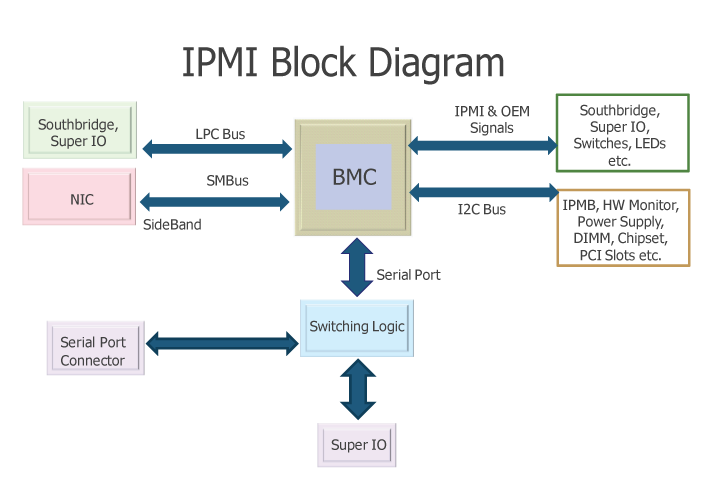
\includegraphics[height=7.5cm]{Imagens/IPMI-Block-Diagram.png}
\caption{Diagrama do IMPI}{Imagem retirada de \protect\url{https://pt.wikipedia.org/wiki/Intelligent_Platform_Management_Interface}, são mostrado os principais componentes do IPMI e como eles se comunicam}
\label{fig:IPMI}
\end{figure}

O  acesso a rede do IPMI pode ser feito pelo protocolo HTTP ou por uma ferramenta disponibilizada pelo fabricante (ipmitool), que também realiza o acesso via rede. Ele também é utilizado para monitorar o status da plataforma com um conjunto de sensores acoplados como temperaturas do sistema, tensões, ventiladores e fontes de alimentação.

\subsection{RAPL}

Microprocessadores Intel modernos, a partir da arquitetura SandyBridge, incluem a interface RAPL \cite{Rotem2012, Hahnel2012, Hackenberg2015} projetada para limitar o uso de energia em um chip ao mesmo tempo que garante o máximo desempenho. Essa interface suporta recursos de medição de energia através de um circuito integrado que estima o uso de energia com base em um modelo conduzido por contadores de eventos arquiteturais de todos os componentes. Além disso também fornece leituras de temperatura e modelos de vazamento de corrente. As estimativas são disponibilizadas em registradores específico de modelo \abrv[MSR -- Model Specific Register]{(MSR)}, sendo atualizado na ordem de milissegundos. As estimativas de energia oferecidas pela RAPL foram validadas pela Intel que mostrou ótimos resultados.
	
	% Capítulo 2
\chapter{Revisão Bibliografia} \label{cap:revisao_bibliografica}

O DVFS é a técnica mais comum empregada para obter economia de energia em sistemas com processadores modernos. Assim, a técnica tem sido extensivamente pesquisada com o objetivo de fornecer estratégias para selecionar a tensão e a frequência ideais para uma aplicação em arquitetura específica. Existem diversas teorias sobre a melhor forma de aplicá-la. No artigo \cite{Albers2014} foi provado que o problema de escalonamento de frequência com o estado ocioso para minimizar a energia é da classe NP-difícil. Embora seja complicado encontrar a melhor configuração possível, com algumas simplificações no modelo é possível encontrar bons resultados, sendo um problema  no qual não existe uma solução ótima.

Em \cite {Anghel2011}, os autores utilizaram dois algoritmos para escalonar a frequência dos processadores: um algoritmo inspirado no sistema imunológico humano para monitorar os estados de potência e desempenho do servidor e um algoritmo baseado em lógica fuzzy para alterar o estado de desempenho do servidor. Também em \cite{Cochran2011} foi introduzido um método de escalonamento para determinar os pontos de operação ideais do sistema para o número de núcleos e configurações de DVFS.

\cite{DaCosta2015} propôs uma abordagem que considera estados de atividade instantânea do sistema, nesse caso, a memória e a atividade de rede foram usadas para gerar uma configuração de gerenciamento de DVFS. 

Registradores contadores de performance do RAPL também foram usados para executar o DVFS. Em \cite{Spiliopoulos2011}, os autores usaram um DVFS contínuo adaptável com base em um modelo de desempenho do processador. O modelo foi baseado na amostragem de contadores de desempenho em hardware para ver regularmente cargas de trabalho de desempenho/energia. Baseando-se nas predições as configurações apropriadas de voltagem e as frequências eram selecionadas.

\cite{Georgiou:2017} utilizaram um modelo de energia para uma arquitetura multissegmentada de vários núcleos e análise de recursos estáticos para avaliar a economia de energia e tempo de várias configurações de DVFS para o mesmo programa. Embora tenham sido capazes de identificar a melhor configuração sem a necessidade de executar o programa com cada configuração diferente e medir tempo e energia, a abordagem é bastante limitada, pois a análise estática não é dimensionada para arquiteturas e programas menos previsíveis.


Com base no que já foi pesquisado foi percebido que modelagem de potencia e desempenho de aplicações não são utilizados para o DVFS, que é a proposta deste trabalho. Além disso o foco do DVFS é redução do consumo de potência o que pode levar a um maior consumo de energia devido ao aumento no tempo total de execução. Outro problema é quando existe variações bruscas na carga do processador que causam uma variação muito grande na frequência que geralmente não leva a bons resultados.

	% Capitulo 3: Terceiro capítulo (arquivo Includes/Capitulo3.tex)
	% Capítulo 4
\chapter{Modelos} \label{cap:modelos}

\section{Potência}  \label{sec:potencia}

Os principais fatores que contribuem para o consumo de energia do processador são consumo dinâmico, por curto-circuito e a perda de energia devido ao vazamento de corrente \cite{Rauber2014, Goel2016, Du2017, Gonzalez1997}, sendo que, a complexidade dos circuitos dos processadores modernos torna muito difícil modelar seu consumo de energia fisicamente acurado. Uma abordagem viável para modelar o consumo de energia do processador é modelar seus componentes principais, que são as portas lógicas. Assim, modelar o consumo de energia para uma porta lógica e multiplicando pelo número total de portas, reduz a complexidade da modelagem e fornecendo precisão suficiente para tomar decisões de otimização, que pode ser observado na seção \ref{cap:resultados}.

A modelagem do consumo de energia do processador utilizada baseia-se no circuito \abrv[CMOS -- Complementary Metal Oxide Semiconductor]{CMOS} \cite{Sarwar1997, Butzen2007} que é uma tecnologia empregada na fabricação de circuitos lógicos. Esta modelagem é uma aproximação que leva em consideração que o processador é basicamente constituído destes circuitos. Sendo assim, o consumo total de energia é proporcional ao número de circuitos lógicos multiplicado pelo consumo de um circuito lógico.

Existem 3 componentes principais para a dissipação de energia nos circuitos CMOS como visto na Equação (\ref{eq_totalPower}).

\begin{equation}
P_{total}=P_{static}+P_{leak}+P_{dynamic} \label{eq_totalPower}
\end{equation}

Onde $P_{total}$ é a potência total dissipada, $P_{dynamic}$ é a dinâmica, devido ao chaveamento do circuito, $P_{static}$ a potência estática e $P_{leak}$ e a potência  perdida devido ao vazamento de corrente no transistor.

Na Figura \ref{fig:CMOS} é mostrado um circuito CMOS inversor que é composto por dois transistores um PMOS e un NMOS, e mais um capacitor.

\begin{figure}[H]
\centering
\includegraphics[height=7.5cm]{Imagens/CMOS.jpg}
\caption{Diagrama eletrico do circuito do CMOS inversor}{Imagem retirada de \protect\url{https://www.hindawi.com/journals/vlsi/2012/505983/}}
\label{fig:CMOS}
\end{figure}

A dissipação de potência dinâmica é causada pela carga do capacitor no circuito durante cada transição de alto para baixo na tensão de entrada, onde parte da energia da fonte é dissipada no PMOS e a outra parte é armazenada no capacitor que é descarregada no NMOS na transição de baixo para alta, na tensão de entrada.

Considerando o CMOS inversor mostrado na Figura \ref{fig:CMOS}, assumindo que a tensão de entrada tem a forma de uma onda quadrada com período de ciclo de trabalho T a energia consumida na transição baixo para alto pode ser derivada calculando a potência média consumida pela fonte o que é dado por (\ref{eq:pwdyn}).

\begin{equation}
P_{dynamic}=\frac{1}{\delta T}\int_{t_1}^{t_2}P(t)dt=\frac{1}{T}\int_{0}^{\infty}i_{vdd}(t)V_{dd}dt \label{eq:pwdyn}
\end{equation}

Sabendo que a corrente em um capacitor é dada por \ref{eq:corrent_cap}.

\begin{equation}
i_{vdd}=C\frac{dV}{dt} \label{eq:corrent_cap}
\end{equation}

Assim temos (\ref{eq:pwdyn_2}).

\begin{equation}
P_{dynamic}=\frac{V_{dd}}{T}\int_{0}^{\infty}C\frac{dV}{dt}dt=\frac{CV_{dd}^2}{T}=CV_{dd}^2f \label{eq:pwdyn_2}
\end{equation}

A corrente vazada no circuito é devido principalmente a diversos fatores como visto em \cite{Butzen2007}, mas como a variação da corrente de vazamento é pequena para simplificar consideraremos que a corrente vazada é praticamente constante simplificando para (\ref{eq:pwleak}):

\begin{equation}
P_{leak}=I_{leak}V_{dd}\alpha V_{dd} \label{eq:pwleak}
\end{equation}

A potência estática é devido a corrente que vai da fonte diretamente para o terra que é aproximadamente constante.

Embora seja possível alterar a frequência e voltagem de forma independente, na prática isso não acontece \cite{Usman2013}, pois dado uma voltagem existe uma frequência máxima em que o circuito pode chegar, para a qual acima deste valor os resultados já não são mais confiáveis. Essa frequência é limitada pelo caminho crítico do circuito, que é a maior distancia entre uma entrada e saída. Também, a frequência nunca é colocada em um valor muito baixo pois resultaria em desperdício de energia. Logo os circuitos tendem a seguir a relação (\ref{eq:fpropv_1}).

\begin{equation}
f \alpha \frac{(V-V_{th})^{\eta}}{V} \label{eq:fpropv_1}
\end{equation}
%\simb[$\alpha$ Proporcional]{$\alpha$}

Onde $V_{th}$ é a voltagem de transição, $\eta$ é uma constante que depende da resposta em frequência do transistor. Para os transistor que não saturam com velocidade podemos considerar $V>>V_{th}$ e aproximar $n=2$ segundo \cite{Gonzalez1997}.

\begin{equation}
f \approx \frac{(V-V_{th})^{\eta}}{V} \approx \frac{V^2}{V} \approx V  \label{eq:fpropv_2}
\end{equation}

Assim o modelo final do processador considerando que ele tem n circuitos lógicos é (\ref{eq:final_1}).

\begin{equation}
P_{total}(f)= (CV_{dd}^2f+I_lV_{dd}+P_s)n \label{eq:final_1}
\end{equation}

Simplificando as constantes e colocando tudo em função da frequência temos (\ref{eq:final_fit}).

\begin{equation}
P_{total}(f)= c_1f^3+c_2f+c_3 \label{eq:final_fit}
\end{equation}

Ampliando este modelo de forma eurística para sistemas multicores com p cores, foi definido (\ref{eq:final_cores}).

\begin{equation}
P_{total}(f,p)= p(c_1f^3+c_2f)+c_3 \label{eq:final_cores}
\end{equation}

Finalmente, considerando sistemas com mais de um processador, onde foi incluído mais um termo estático devido a energia para ativar cada um, resultando em (\ref{eq:final_cores_sock}).

\begin{equation}
P_{total}(f,p,s)= p(c_1f^3+c_2f)+c_3+c_4s \label{eq:final_cores_sock}
\end{equation}

Onde $s$ é o número total de processadores, $p$ é o numero de núcleos, $f$ a frequência e $c_1$,$c_2$,$c_3$ e $c_4$ são constantes.

\section{Performance} \label{sec:performance}

O modelo de performance tem como objetivo estimar o tempo de execução da aplicação a partir da frequência, número de cores e tamanho da entrada. Para isso foi utilizado a SVR como visto na Figura \ref{fig:svr}, que é uma versão da técnica de aprendizagem da máquina supervisionada baseada em vetor de suporte para regressão.

\begin{figure}[H]
\centering
\includegraphics[height=2cm]{Imagens/svr_diagrama.png}
\caption{Diagrama da SVR}
\label{fig:svr}
\end{figure}

A SVR \cite{Drucker1997} consiste em encontrar uma função $f(x)$ de forma que o erro máximo para o alvo seja de $\epsilon$ para todos os pontos do treinamento \cite{Smola2004}. Ela funciona da seguinte forma: Dado o conjunto de treinamento, um vetor de entrada $x_i$ com saída $y_i$, é resolvido o seguinte problema de otimização (\ref{eq:svr_primal}).

\begin{equation}
\label{eq:svr_primal}
\min_{w,\xi_i,\xi_i^*}\frac{1}{2}w^Tw+C\sum_{i}^{n}{\xi_i+\xi_i^*}
\end{equation}
Sujeito a:
\[ 
\begin{cases} 
      y_i-w^T\phi(x_i)-b \leq \varepsilon+\xi_i \\
      w^T\phi(x_i)+b-y_i \leq \varepsilon+\xi_i^* \\
      \xi_i,\xi_i^* \geq 0, i=0,..,n
\end{cases}
\]

Os valores que queremos encontrar são $w$ que é o vetor de suporte. $\xi$ é uma variável de folga que permite que o modelo tenha um erro maior que $\epsilon$ em alguns casos, garantindo a convergência onde existem pontos muito fora da curva e b que é o bias.

Os parâmetros desse modelo são, $\phi(x)$, $\epsilon$ e $C$. O $\phi(x)$ é uma função kernel que mapeia a entrada em outro espaço de maior dimensão permitindo que o algoritmo se ajuste ao hiperplano de margem máxima em um espaço transformado. Isso permite a não linearidade desse algoritmo ao utilizar uma função kernel não linear. As funções kernel mais comuns são polinomial, função de base radial de Gauss (RBF) e tangente hiperbólica. O $\epsilon$ é o desvio máximo para o alvo $y_i$. A constante $C$ determina a tolerância para erros maiores que $\epsilon$.

A resolução deste problema de otimização pode ser feita eficientemente em sua forma dual de Lagrange, que é obtida através da função objetivo de Lagrange utilizando multiplicadores não negativos. Ao adicionar as restrições de otimização e resolver para as variáveis do problema original que minimiza esta função ficando com as variáveis do problema original em função dos multiplicadores de Lagrange, que são chamados de variáveis duais, assim o novo problema é maximizar a função objetivo em função das variáveis duais incluindo as restrições de não negatividade. O novo problema se torna:

\begin{equation}
\label{eq:svr_dual}
\max_{\alpha,\alpha^*}{-\frac{1}{2}\sum_{i,j}{(\alpha_i-\alpha_i^*)(\alpha_j-\alpha_j^*)k(x_i,x_j)}-\epsilon \sum_{i}{(\alpha_i-\alpha_i^*)}+\sum_{i}{y_i(\alpha_i-\alpha_i^*)}}
\end{equation}
Sujeito a:
\[
\begin{cases} 
      \sum_{i}{(\alpha_i-\alpha_i^*)}=0\\
      \alpha_i,\alpha_i^* \in [0,C] \\
   \end{cases}
\]

Onde $k(x,x')=\langle \phi(x), \phi(x') \rangle$ e $\alpha_i,\alpha_i^*$ são os multiplicadores de Lagrange e $f(x)$,$w$ e $b$ são:

\begin{equation}
\label{eq:svr_fx}
f(x)= \sum_{i}{(\alpha_i-\alpha_i^*)k(x_i,x)}+b
\end{equation}

\begin{equation}
\label{eq:svr_w}
w= \sum_{i}{(\alpha_i-\alpha_i^*)\phi(x_i)}
\end{equation}

\begin{equation}
\label{eq:svr_b}
b= y_i-\langle w,x_i \rangle-\epsilon
\end{equation}

Os valores de $\alpha_i,\alpha_i^*$ por sua vez podem ser encontrados de forma iterativa e eficiente utilizando o algorítimo "Sequential minimal optimization" \cite{Platt1998}.

Pela equação (\ref{eq:svr_fx}) podemos ver que a complexidade do algorítimo é linearmente dependente do número de amostras do treinamento assim como os vetores de suporte. A grande vantagem desse método é que pelas restrições do problema de otimização serem estritamente convexas, é garantida uma solução única. Isto significa que algorítimos SVs não tem problemas de mínimos locais como Redes Neurais.


\section{Energia} \label{sec:energia}

Combinando o modelo de energia da seção anterior e a caracterização SVR do tempo podemos estimar a energia total consumida com a equação da energia média descrita por:

\begin{equation}
%E_m=\int_{t1}^{t2}P_mdt=P_m\delta T
E_m=P_m\Delta T
\end{equation}

Substituindo os modelos descritos nas Seções \ref{sec:potencia} e \ref{sec:performance}, obtemos a equação (\ref{eq:energia}).

\begin{equation}
E(f,p,s,N)=P(f,p,s)SVR(f,p,N)
\label{eq:energia}
\end{equation}

Onde $f$ é a frequência, $p$ o número de cores ativos, $s$ o número de processadores ativos e $N$ o tamanho da entrada.

Este modelo possui algumas restrições, pois, não prevê a variação do consumo de potência ao longo do tempo, devido à variação da utilização do processador. Assim é necessário escolher uma carga para modelar a equação de potência. Por causa disso a energia real consumida será diferente da estimada por um fator multiplicativo em alguns casos, mas, a tendência geral será a mesma, o que possibilita encontrar o mínimo.

Com esta equação é possível encontrar a configuração onde a energia é minimizada para uma determinada entrada, mas, também encontrar a configuração mínima de energia dada uma restrição de tempo, frequência ou número de núcleos ativos.	
	
	% Capitulo 4: Quarto capítulo (arquivo Includes/Capitulo4.tex)
	% Capítulo 3
\chapter{Metodologia} \label{cap:metodologia}

\section{Configuração} \label{sec:config}
Nos experimentos realizados neste trabalho, foi utilizado um nó de computação que consiste em dois processadores Intel Xeon E5-2698 v3 com dezesseis núcleos e duas threads de hardware para cada núcleo. A frequência máxima não turbo de 2.3 GHz e a memória física total do nó é de 128 GB (8 $ \times $ 16 GB) com o sistema operacional CentOS 6.5 e kernel Linux  versão 4.16. A frequência turbo e o hyper-thread foram desativados durante todos os experimentos.


\section{Aplicações} \label{sec:apps}

O processo de caracterização foi realizado utilizando aplicações do PARSEC benchmark que possui uma suíte de aplicações paralelas que foi projetado para ser representativo da próxima geração de programas de memória compartilhada em chips com múltiplos processadores. As aplicações do PARSEC cobrem as mais diversas áreas, tais como, análise de finanças, visão computacional, mineração de dados, aprendizagem de máquina e processamento de mídia, variando no tipo de paralelização, intensidade de comunicação e tamanho do problema de entrada. Neste trabalho foram utilizadas as aplicações Blackscholes, Fuidanimate, Raytrace e Swaptions da versão 3.0.

\begin{itemize}
	
	\item Blackscholes: calcula os preços de uma carteira de opções européias analiticamente com a equação diferencial parcial de Black-Scholes. Não há expressão em forma fechada para a equação de Black-Scholes e, como tal, deve ser calculada numericamente. Suas entradas são número de threads, arquivo de entrada contendo os dados das opções e nome do arquivo de saída.
	
	\item Fuidanimate: usa uma extensão do método de hidrodinâmica de partículas suavizadas (SPH) para simular um fluido incompressível para fins de animação interativa. Suas entradas são o número de threads do número de quadros e um arquivo de entrada com informações de todas as partículas fluidas e suas propriedades.
	
	\item O Raytrace: uma versão do método de raytracing que normalmente seria empregada para animações em tempo real, como jogos de computador. Está otimizado para a velocidade e não para o realismo. A complexidade computacional do algoritmo depende da resolução da imagem de saída e da cena. As entradas usadas nesses aplicativos são o número de threads, o número de quadros, um objeto 3D e a resolução da tela.
	
	\item Swaptions: utiliza o framework Heath-Jarrow-Morton para calcular os preços do portifolio swaptions. Swaptions emprega simulações de Monte Carlo para computar os preços. A entrada para este programa é o número de threads, swaptions e tentativas. 
	
\end{itemize}

\section{Ajuste do modelo de potência} \label{sec:met_ajuste_pw}

Para encontrar as constantes, foram desenvolvidas aplicações que utilizam todo o tempo do processador com diversas instruções diferentes, pois, dependendo da instrução executada, pode variar o consumo do processador.

Com essas aplicações foram coletadas amostras de frequência com RAPL e IPMI durante sua execução, variando a frequência de 1.2 GHz até 2.3 GHz, com passos de 100 MHz, e o número de núcleos de 2 até 32, com um passo de 2. A taxa de amostragem foi de aproximadamente 1 segundo e o tempo de execução de 2 a 5 minutos. Entre cada teste foi esperado um tempo de 30 segundos para as próximas medições não serem afetadas pelas anteriores. Com esses dados foi feita uma regressão multi-linear com o método dos mínimos quadrados para descobrir os coeficientes da equação de potência descrito na Seção \ref{sec:potencia}. Que se resume a resolver a equação $\vec{c}=(A^TA)^{-1}A^TB$, onde $\vec{c}$ é o vetor dos coeficientes da equação $A\vec{c}=B$, onde:

\begin{equation}
A=
\begin{bmatrix}
p_1f_1^3 & p_1f_1 & 1 & s_1 \\
p_2f_2^3 & p_1f_2 & 1 & s_1 \\
& \vdots \\
p_nf_m^3 & p_nf_m & 1 & s_2 \\
\end{bmatrix}
\quad e\quad B= 
\begin{bmatrix}
P_1 \\
P_2 \\
\vdots \\
P_k
\end{bmatrix}
\end{equation}

Para cada valor de frequência $f_i$ e número de núcleos $p_i$ associados a potencia $P_i$.

Para validar este modelo foi calculado a média do erro percentual \abrv[MEP -- Média do erro percentual]{(MEP)} e o erro médio absoluto \abrv[MEA -- Média do erro absoluto]{(MEA)}. Essas métricas foram escolhida devido à diferença significativa entre o menor e maior valor. Elas são descritas por (\ref{eq:mpe}).

\begin{equation}
MEP=\frac{1}{n_{amostras}}\sum_{i}^{n_{amostras}}{\frac{|y_i-y_{\rm model}|}{y_i}} \quad MEA=\frac{1}{n_{amostras}}\sum_{i}^{n_{amostras}}{|y_i-y_{\rm model}|}
\label{eq:mpe}
\end{equation}


\section{Treinamento do modelo de performance} \label{sec:met_ajuste_perf}

Para caracterizar a aplicação, foram coletados o tempo de execução para diferentes configurações de números de núcleos ativos dentro do intervalo de $ 1 <= p <= 32 $, e frequência no intervalo de $ 1,2 <= f <= 2,2 $ GHz, com passos de 100 MHz para 5 tamanhos de entradas diferentes, que por sua vez foram escolhidos de forma a dobrar o tamanho do problema a cada entrada, seguindo a equação:

\begin{equation}
N(x)=\frac{M}{2^{p-x}}, 0<x\leq p
\end{equation}

Em que M é o maior problema e p é o numero de divisões. Assim a complexidade resultante do tempo do algoritmo é dado por $O(N(x))$. O tempo médio de execução foi da ordem de minutos. E ao mesmo tempo que era registrado o tempo de execução, também eram coletadas amostras de energia a cada segundo, para futuras comparações com o modelo proposto.

Foi utilizado o método busca em grid para encontrar os melhores parâmetros para o modelo. Ele procura entre vários valores especificados os que apresentam melhores resultados. Neste caso, um kernel de função de base radial \abrv[RBF -- Radial Base Funtion]{(RBF)} dado pela Equação $\phi(r)=e^{-(\gamma r)^2}$ com $\gamma=0.5$. A penalidade por termo errado foi $C=10^4$. A implementação utilizada foi a da biblioteca scikit-learn \cite{scikit-learn}. Para treinar o SVR, os dados coletados foram divididos em duas partes, 90 \% para treinamento e 10 \% para teste. O tempo total para coletar os dados da caracterização variou entre algumas horas e 1 dia, dependendo da aplicação.

% \begin{equation}
% \label{eq:rbf}
% \phi(r)=e^{-(\gamma r)^2}
% \end{equation}

O modelo foi validado com uma validação cruzada do tipo fold com 10 divisões, usando MEA e o MEP como métricas.
	
	% Capitulo 5: Quinto capítulo (arquivo Includes/Capitulo5.tex)
	% Capítulo 5
\chapter{Resultados} \label{cap:resultados}

Nesta sessão serão mostrados os ajustes dos modelos e o resultado do modelo final de energia.

\section{Modelo de potência}

O modelo de potencia ajustado pode ser visto na Figura \ref{fig:pot_ipmi} e os parâmetros da equação em (\ref{eq:fittedpower}) com a unidade de frequência em GHz.

\begin{figure}[H]
\centering
\includegraphics[height=8cm]{Imagens/potencia_ipmi.png}
\caption{Ajuste Modelo de Potencia}{Onde os pontos representam os valores reais de potência medidos com o IPMI e a grade a curva obtida}
\label{fig:pot_ipmi}
\end{figure}

\begin{equation} 
P_{total}(f,p,s)=p(0.29f^3+0.97f)+198.59+9.18s \label{eq:fittedpower}
\end{equation}

O MEP resultante foi de 0.75\% e MEA foi de 1.89W.

\section{Modelo de performance} \label{sec:ajuste_perf}

Alguns resultados da caracterização podem ser vistos na Figura \ref{fig:tempos} onde é mostrada a curva obtida pela SVR e os valores reais medidos.

\begin{figure}[H]
	\centering
	\begin{subfigure}[t]{0.5\textwidth}
		\centering
		\includegraphics[width=\columnwidth]{Imagens/time/black_3.png}
		\caption{Tempo Blackscholes}
	\end{subfigure}%
	~ 
	\begin{subfigure}[t]{0.5\textwidth}
		\centering
		\includegraphics[width=\columnwidth]{Imagens/time/fluid_3.png}
		\caption{Tempo Fluidanimate}
	\end{subfigure}
	\\
	\centering
	\begin{subfigure}[t]{0.5\textwidth}
		\centering
		\includegraphics[width=\columnwidth]{Imagens/time/swap_3.png}
		\caption{Tempo Swaptions}
	\end{subfigure}%
	~
	\begin{subfigure}[t]{0.5\textwidth}
		\centering
		\includegraphics[width=\columnwidth]{Imagens/time/rtview_3.png}
		\caption{Tempo Raytrace}
	\end{subfigure}
	
	\caption{Tempo para modelo de performance}
	\label{fig:tempos}
\end{figure}

A media dos  resultados da validação cruzada podem ser vistos na Tabela \ref{tab:svr_evaluation}.

\begin{table}[H]
\centering
\begin{tabular}{|l|l|l|l|l|}
\hline
\hline
Application  & MEA & MEP \\ \hline
Blackscholes & 2.01  & 4.6\% \\ \hline
Fluidanimate & 6.65  & 1.89\% \\ \hline
Raytrace  & 3.77  & 0.87\% \\ \hline
Swaptions & 2.29  & 2.56\% \\ \hline
\end{tabular}
\caption{Performance-Model's Cross validation Errors}
\label{tab:svr_evaluation}
\end{table}


\section{Energia} \label{sec:ajuste_en}

As Figuras \ref{fig:energia_black}, \ref{fig:energia_fluid}, \ref{fig:energia_rtview} e \ref{fig:energia_swaptions} mostram os valores de energia medidos junto com a superfície ajustada do modelo. As medições de energia foram obtidas integrando a potência ao longo do tempo total de execução da aplicação.

\begin{figure}[H]
    \centering
    \begin{subfigure}[t]{0.5\textwidth}
        \centering
        \includegraphics[width=\columnwidth]{Imagens/energy/black_1.png}
        \caption{Entrada 1}
    \end{subfigure}%
    ~ 
    \begin{subfigure}[t]{0.5\textwidth}
        \centering
        \includegraphics[width=\columnwidth]{Imagens/energy/black_2.png}
        \caption{Entrada 2}
    \end{subfigure}
    \\
    \centering
    \begin{subfigure}[t]{0.5\textwidth}
        \centering
        \includegraphics[width=\columnwidth]{Imagens/energy/black_3.png}
        \caption{Entrada 3}
    \end{subfigure}%
    ~ 
    \begin{subfigure}[t]{0.5\textwidth}
        \centering
        \includegraphics[width=\columnwidth]{Imagens/energy/black_4.png}
        \caption{Entrada 4}
    \end{subfigure}
    \\
    \centering
    \begin{subfigure}[t]{0.5\textwidth}
        \centering
        \includegraphics[width=\columnwidth]{Imagens/energy/black_5.png}
        \caption{Entrada 5}
    \end{subfigure}%
    ~ 
    \begin{subfigure}[t]{0.5\textwidth}
        \centering
        \includegraphics[width=\columnwidth]{Imagens/energy/black_6.png}
        \caption{Entrada 6}
    \end{subfigure}
	\caption{Modelo de Energia do Blackscholes}
	\label{fig:energia_black}
\end{figure}

\begin{figure}[H]
    \centering
    \begin{subfigure}[t]{0.5\textwidth}
        \centering
        \includegraphics[width=\columnwidth]{Imagens/energy/fluid_1.png}
        \caption{Entrada 1}
    \end{subfigure}%
    ~ 
    \begin{subfigure}[t]{0.5\textwidth}
        \centering
        \includegraphics[width=\columnwidth]{Imagens/energy/fluid_2.png}
        \caption{Entrada 2}
    \end{subfigure}
    \\
    \centering
    \begin{subfigure}[t]{0.5\textwidth}
        \centering
        \includegraphics[width=\columnwidth]{Imagens/energy/fluid_3.png}
        \caption{Entrada 3}
    \end{subfigure}%
    ~ 
    \begin{subfigure}[t]{0.5\textwidth}
        \centering
        \includegraphics[width=\columnwidth]{Imagens/energy/fluid_4.png}
        \caption{Entrada 4}
    \end{subfigure}
    \\
    \centering
    \begin{subfigure}[t]{0.5\textwidth}
        \centering
        \includegraphics[width=\columnwidth]{Imagens/energy/fluid_5.png}
        \caption{Entrada 5}
    \end{subfigure}%
    ~ 
    \begin{subfigure}[t]{0.5\textwidth}
        \centering
        \includegraphics[width=\columnwidth]{Imagens/energy/fluid_6.png}
        \caption{Entrada 6}
    \end{subfigure}
    
    \caption{Modelo de Energia do Fluidanimate}
    \label{fig:energia_fluid}
\end{figure}

O FluidAnimate possui uma restrição quanto ao número de núcleos que precisa ser potência de 2, assim não temos as mesmas variações das aplicações anteriores mas apresentou comportamento similar, sendo que o decaimento no consumo de energia foi mais gradual com o número de núcleos.

Podemos observar um decaimento do tipo $\frac{1}{p}$ com o numero de núcleos ativos devido ao tempo paralelo seguir essa relação com o tempo serial $T_{paralelo} \alpha \frac{T_{serial}}{p}$, isso mostra a importância da paralelização na economia de energia.

\begin{figure}[H]
    \centering
    \begin{subfigure}[t]{0.5\textwidth}
        \centering
        \includegraphics[width=\columnwidth]{Imagens/energy/swap_1.png}
        \caption{Entrada 1}
    \end{subfigure}%
    ~ 
    \begin{subfigure}[t]{0.5\textwidth}
        \centering
        \includegraphics[width=\columnwidth]{Imagens/energy/swap_2.png}
        \caption{Entrada 2}
    \end{subfigure}
    \\
    \centering
    \begin{subfigure}[t]{0.5\textwidth}
        \centering
        \includegraphics[width=\columnwidth]{Imagens/energy/swap_3.png}
        \caption{Entrada 3}
    \end{subfigure}%
    ~ 
    \begin{subfigure}[t]{0.5\textwidth}
        \centering
        \includegraphics[width=\columnwidth]{Imagens/energy/swap_4.png}
        \caption{Entrada 4}
    \end{subfigure}
    \\
    \centering
    \begin{subfigure}[t]{0.5\textwidth}
        \centering
        \includegraphics[width=\columnwidth]{Imagens/energy/swap_5.png}
        \caption{Entrada 5}
    \end{subfigure}%
    ~ 
    \begin{subfigure}[t]{0.5\textwidth}
        \centering
        \includegraphics[width=\columnwidth]{Imagens/energy/swap_6.png}
        \caption{Entrada 6}
    \end{subfigure}
    
    \caption{Modelo de Energia do Swaptions}
    \label{fig:energia_swaptions}
\end{figure}

\begin{figure}[H]
    \centering
    \begin{subfigure}[t]{0.5\textwidth}
        \centering
        \includegraphics[width=\columnwidth]{Imagens/energy/rtview_1.png}
        \caption{Entrada 1}
	    \label{fig:energia_rtview_e1}
    \end{subfigure}%
    ~ 
    \begin{subfigure}[t]{0.5\textwidth}
        \centering
        \includegraphics[width=\columnwidth]{Imagens/energy/rtview_2.png}
        \caption{Entrada 2}
        \label{fig:energia_rtview_e2}
    \end{subfigure}
    \\
    \centering
    \begin{subfigure}[t]{0.5\textwidth}
        \centering
        \includegraphics[width=\columnwidth]{Imagens/energy/rtview_3.png}
        \caption{Entrada 3}
        \label{fig:energia_rtview_e3}
    \end{subfigure}%
    ~ 
    \begin{subfigure}[t]{0.5\textwidth}
        \centering
        \includegraphics[width=\columnwidth]{Imagens/energy/rtview_4.png}
        \caption{Entrada 4}
        \label{fig:energia_rtview_e4}
    \end{subfigure}
    \\
    \centering
    \begin{subfigure}[t]{0.5\textwidth}
        \centering
        \includegraphics[width=\columnwidth]{Imagens/energy/rtview_5.png}
        \caption{Entrada 5}
        \label{fig:energia_rtview_e5}
    \end{subfigure}%
    ~ 
    \begin{subfigure}[t]{0.5\textwidth}
        \centering
        \includegraphics[width=\columnwidth]{Imagens/energy/rtview_6.png}
        \caption{Entrada 6}
        \label{fig:energia_rtview_e6}
    \end{subfigure}
    
    \caption{Modelo de Energia do RayTrace}
    \label{fig:energia_rtview}
\end{figure}


Podemos perceber que a tendencia foi seguida corretamente, tendo uma maior distorção apenas nas primeiras entradas do Raytrace visto nas figuras \ref{fig:energia_rtview_e1},\ref{fig:energia_rtview_e2},\ref{fig:energia_rtview_e3}.

\section{Comparação de Energia} \label{sec:comp}

Para descobrir a verdadeira economia do método proposto ele foi comparando o consumo de energia das quatro aplicações de estudo de caso. Usando as configurações ótimas de energia fornecidas pela abordagem proposta com o DVFS padrão do Linux, o Ondemand e com o Intel P-state, variando o número de núcleos ativos com os valores de 1 a 32 de forma exponencial e expondo os melhores casos dos 3 métodos, para termos uma melhor ideia de comparação, são mostrados nas tabelas os valores absolutos de consumo, a frequência media e a economia com relação ao modelo proposto.

\begin{table}[H]
	\resizebox{\columnwidth}{!}{
		\begin{tabular}{l|l|l|l|l|l|l|ll}
			\multicolumn{1}{l|}{\rot{Entrada}} & \rot{\begin{tabular}[c]{@{}l@{}}Freq. Media \\ em GHz \\ (\#Cores) \end{tabular}}  & \rot{Energia em KJ}   &  \rot{\begin{tabular}[c]{@{}l@{}}Freq. Media \\ em GHz \\ (\#Cores) \end{tabular}} & \rot{Energia em KJ}  & \rot{\begin{tabular}[c]{@{}l@{}} Freq. \\ em GHz \\ (\#Cores) \end{tabular}} & \rot{Energia em KJ}        & \multicolumn{1}{l|}{\rot{\begin{tabular}[c]{@{}l@{}} Economia \\ Ondemand \end{tabular}}} & \multicolumn{1}{l}{\rot{\begin{tabular}[c]{@{}l@{}} Economia \\ Intel\end{tabular}}} \\ \hline
			\multicolumn{1}{l|}{1} & 1.31 (32) & 0.66 & 1.27 (32) & 0.72 & 1.50 (32)  & 0.97 & \multicolumn{1}{l|}{-32.18} & \multicolumn{1}{l}{-25.89} \\ \hline
			\multicolumn{1}{l|}{2} & 1.20 (32) & 2.18 & 2.80 (32) & 1.67 & 2.10 (28)  & 1.67 & \multicolumn{1}{l|}{30.68} & \multicolumn{1}{l}{0.19} \\ \hline
			\multicolumn{1}{l|}{3} & 2.33 (32) & 3.22 & 2.09 (32) & 3.53 & 2.20 (32)  & 2.97 & \multicolumn{1}{l|}{8.40} & \multicolumn{1}{l}{18.66} \\ \hline
			\multicolumn{1}{l|}{4} & 1.42 (32) & 7.44 & 2.00 (32) & 6.46 & 2.20 (28)  & 6.52 & \multicolumn{1}{l|}{14.11} & \multicolumn{1}{l}{-0.84} \\ \hline
			\multicolumn{1}{l|}{5} & 1.20 (32) & 15.40 & 2.42 (32) & 12.57 & 2.20 (28)  & 13.33 & \multicolumn{1}{l|}{15.48} & \multicolumn{1}{l}{-5.69} \\ \hline
			\multicolumn{1}{l|}{6} & 1.54 (32) & 26.98 & 1.77 (32) & 26.48 & 2.20 (30)  & 25.73 & \multicolumn{1}{l|}{4.85} & \multicolumn{1}{l}{2.89} \\ \hline
			& \multicolumn{2}{l|}{Ondemand Min.} & \multicolumn{2}{l|}{Intel Min.} & \multicolumn{2}{l|}{Proposta} & Economia em \% & \\ 
		\end{tabular}
	}
	\caption{Comparação energia miníma Blackscholes}{Comparação do método proposto com Ondemand e P-state, mostrando a porcentagem de economia com relação aos melhores valores encontrados, onde positivo significa economia.}
	\label{tab:Blackscholesfreq}
\end{table}

Na Tabela \ref{tab:Blackscholesfreq} podemos ver que na maioria das vezes foi obtida configurações que consumiu menos energia, chegando a economia de até 30\%. Apenas para a primeira entrada onde tem o menor tempo de execução a configuração proposta não compensou. A número de núcleos ativos na melhor configuração sempre foi próximo do máximo, ou seja, 32, mesmo que a aplicação não tenha um decaimento no tempo significativo com o aumento no número de núcleos, isso confirma a importância da paralelização nas aplicações para se obter economia de energia. Outra observação importante e que nem sempre a menor frequência levou ao menor consumo de energia, como podemos ver pelo Ondemand que em para todas as entradas teve um média de frequência menor e foi o que consumiu mais energia dos 3 métodos comparados.

\begin{table}[H]
	\resizebox{\columnwidth}{!}{
		\begin{tabular}{l|l|l|l|l|l|l|ll}
			\multicolumn{1}{l|}{\rot{Entrada}} & \rot{\begin{tabular}[c]{@{}l@{}}Freq. Media \\ em GHz \\ (\#Cores) \end{tabular}}  & \rot{Energia em KJ}   &  \rot{\begin{tabular}[c]{@{}l@{}}Freq. Media \\ em GHz \\ (\#Cores) \end{tabular}} & \rot{Energia em KJ}  & \rot{\begin{tabular}[c]{@{}l@{}} Freq. \\ em GHz \\ (\#Cores) \end{tabular}} & \rot{Energia em KJ}        & \multicolumn{1}{l|}{\rot{\begin{tabular}[c]{@{}l@{}} Economia \\ Ondemand \end{tabular}}} & \multicolumn{1}{l}{\rot{\begin{tabular}[c]{@{}l@{}} Economia \\ Intel\end{tabular}}} \\ \hline
			\multicolumn{1}{l|}{1} & 2.15 (32) & 2.28 & 2.61 (32) & 2.61 & 2.10 (32)  & 2.35 & \multicolumn{1}{l|}{-3.03} & \multicolumn{1}{l}{11.05} \\ \hline
			\multicolumn{1}{l|}{2} & 2.01 (32) & 4.36 & 1.74 (32) & 5.13 & 2.00 (32)  & 4.15 & \multicolumn{1}{l|}{5.00} & \multicolumn{1}{l}{23.71} \\ \hline
			\multicolumn{1}{l|}{3} & 1.68 (32) & 9.00 & 2.22 (32) & 10.01 & 2.00 (32)  & 7.89 & \multicolumn{1}{l|}{14.13} & \multicolumn{1}{l}{26.93} \\ \hline
			\multicolumn{1}{l|}{4} & 1.93 (32) & 16.87 & 2.51 (32) & 18.69 & 2.00 (32)  & 16.98 & \multicolumn{1}{l|}{-0.63} & \multicolumn{1}{l}{10.09} \\ \hline
			\multicolumn{1}{l|}{5} & 1.98 (32) & 33.29 & 2.63 (32) & 37.68 & 2.10 (32)  & 33.20 & \multicolumn{1}{l|}{0.26} & \multicolumn{1}{l}{13.47} \\ \hline
			\multicolumn{1}{l|}{6} & 1.43 (32) & 68.43 & 2.54 (32) & 77.30 & 2.10 (32)  & 66.67 & \multicolumn{1}{l|}{2.65} & \multicolumn{1}{l}{15.95} \\ \hline
			& \multicolumn{2}{l|}{Ondemand Min.} & \multicolumn{2}{l|}{Intel Min.} & \multicolumn{2}{l|}{Proposta} & Economia em \% & \\ 
		\end{tabular}
	}
	\caption{Comparação energia miníma Fluidanimate}{Comparação do método proposto com Ondemand e P-state, mostrando a porcentagem de economia com relação aos melhores valores encontrados, onde positivo significa economia.}
	\label{tab:Fluidanimatefreq}
\end{table}

A comparação do Fluidanimate visto na Tabela \ref{tab:Fluidanimatefreq} foi o que apresentou melhor resultado tendo economia em todos as entradas comparado ao P-state e na maioria contra o Ondemand. A frequência do Ondemand e método proposto foram bem próximas e mesmo assim foi obtido economia isso pode ser explicado pela variação de frequência que existe no Ondemand levando a um maior tempo de execução.

\begin{table}[H]
	\resizebox{\columnwidth}{!}{
		\begin{tabular}{l|l|l|l|l|l|l|ll}
			\multicolumn{1}{l|}{\rot{Entrada}} & \rot{\begin{tabular}[c]{@{}l@{}}Freq. Media \\ em GHz \\ (\#Cores) \end{tabular}}  & \rot{Energia em KJ}   &  \rot{\begin{tabular}[c]{@{}l@{}}Freq. Media \\ em GHz \\ (\#Cores) \end{tabular}} & \rot{Energia em KJ}  & \rot{\begin{tabular}[c]{@{}l@{}} Freq. \\ em GHz \\ (\#Cores) \end{tabular}} & \rot{Energia em KJ}        & \multicolumn{1}{l|}{\rot{\begin{tabular}[c]{@{}l@{}} Economia \\ Ondemand \end{tabular}}} & \multicolumn{1}{l}{\rot{\begin{tabular}[c]{@{}l@{}} Economia \\ Intel\end{tabular}}} \\ \hline
			\multicolumn{1}{l|}{1} & 2.77 (32) & 4.11 & 2.77 (32) & 4.14 & 1.80 (32)  & 4.52 & \multicolumn{1}{l|}{-9.00} & \multicolumn{1}{l}{-8.49} \\ \hline
			\multicolumn{1}{l|}{2} & 2.77 (32) & 6.37 & 2.76 (32) & 6.30 & 2.20 (32)  & 5.73 & \multicolumn{1}{l|}{11.18} & \multicolumn{1}{l}{10.01} \\ \hline
			\multicolumn{1}{l|}{3} & 2.77 (32) & 8.49 & 2.76 (32) & 8.51 & 2.20 (32)  & 7.81 & \multicolumn{1}{l|}{8.73} & \multicolumn{1}{l}{8.91} \\ \hline
			\multicolumn{1}{l|}{4} & 2.58 (32) & 10.59 & 2.71 (32) & 10.61 & 2.00 (32)  & 9.90 & \multicolumn{1}{l|}{6.92} & \multicolumn{1}{l}{7.14} \\ \hline
			\multicolumn{1}{l|}{5} & 2.57 (32) & 12.68 & 2.60 (32) & 12.68 & 2.10 (32)  & 12.01 & \multicolumn{1}{l|}{5.63} & \multicolumn{1}{l}{5.62} \\ \hline
			\multicolumn{1}{l|}{6} & 2.15 (32) & 14.86 & 2.30 (32) & 14.78 & 1.90 (32)  & 14.45 & \multicolumn{1}{l|}{2.86} & \multicolumn{1}{l}{2.29} \\ \hline
			& \multicolumn{2}{l|}{Ondemand Min.} & \multicolumn{2}{l|}{Intel Min.} & \multicolumn{2}{l|}{Proposta} & Economia em \% & \\ 
		\end{tabular}
	}
	\caption{Comparação energia miníma Swaptions}{Comparação do método proposto com Ondemand e P-state, mostrando a porcentagem de economia com relação aos melhores valores encontrados, onde positivo significa economia.}
	\label{tab:Swaptionsfreq}
\end{table}

As configurações ótimas para a aplicação Swaptions mostram resultados de economia similares as aplicações mostradas anteriormente, como visto na Tabela \ref{tab:Swaptionsfreq} podemos ver que na maioria das vezes também foi obtida configurações que consumiu menos energia, e apenas para a primeira entrada a configuração proposta não compensou. Nessa aplicação as frequências médias do Ondemand e P-state foram bem maiores do que o método proposto diferente da aplicação anterior, mesmo assim em ambas as aplicações houve economia de energia no método proposto isso mostra que cada aplicação tem suas configurações ideais não tendo uma configuração que economize em todas.

\begin{table}[H]
	\resizebox{\columnwidth}{!}{
		\begin{tabular}{l|l|l|l|l|l|l|ll}
			\multicolumn{1}{l|}{\rot{Entrada}} & \rot{\begin{tabular}[c]{@{}l@{}}Freq. Media \\ em GHz \\ (\#Cores) \end{tabular}}  & \rot{Energia em KJ}   &  \rot{\begin{tabular}[c]{@{}l@{}}Freq. Media \\ em GHz \\ (\#Cores) \end{tabular}} & \rot{Energia em KJ}  & \rot{\begin{tabular}[c]{@{}l@{}} Freq. \\ em GHz \\ (\#Cores) \end{tabular}} & \rot{Energia em KJ}        & \multicolumn{1}{l|}{\rot{\begin{tabular}[c]{@{}l@{}} Economia \\ Ondemand \end{tabular}}} & \multicolumn{1}{l}{\rot{\begin{tabular}[c]{@{}l@{}} Economia \\ Intel\end{tabular}}} \\ \hline
			\multicolumn{1}{l|}{1} & 1.45 (8) & 32.62 & 3.60 (2) & 31.47 & 2.20 (4)  & 34.37 & \multicolumn{1}{l|}{-5.08} & \multicolumn{1}{l}{-8.43} \\ \hline
			\multicolumn{1}{l|}{2} & 1.54 (16) & 37.06 & 1.78 (16) & 34.39 & 2.20 (6)  & 37.92 & \multicolumn{1}{l|}{-2.26} & \multicolumn{1}{l}{-9.31} \\ \hline
			\multicolumn{1}{l|}{3} & 1.85 (8) & 41.53 & 1.33 (8) & 39.65 & 2.20 (10)  & 39.93 & \multicolumn{1}{l|}{3.99} & \multicolumn{1}{l}{-0.72} \\ \hline
			\multicolumn{1}{l|}{4} & 1.88 (16) & 47.04 & 2.24 (16) & 44.44 & 2.20 (14)  & 45.77 & \multicolumn{1}{l|}{2.78} & \multicolumn{1}{l}{-2.91} \\ \hline
			\multicolumn{1}{l|}{5} & 1.68 (32) & 51.88 & 2.42 (32) & 50.34 & 2.20 (22)  & 52.99 & \multicolumn{1}{l|}{-2.09} & \multicolumn{1}{l}{-5.00} \\ \hline
			\multicolumn{1}{l|}{6} & 2.06 (32) & 65.02 & 2.78 (32) & 65.84 & 2.20 (26)  & 67.28 & \multicolumn{1}{l|}{-3.36} & \multicolumn{1}{l}{-2.14} \\ \hline
			& \multicolumn{2}{l|}{Ondemand Min.} & \multicolumn{2}{l|}{Intel Min.} & \multicolumn{2}{l|}{Proposta} & Economia em \% & \\ 
		\end{tabular}
	}
	\caption{Comparação energia miníma Raytrace}{Comparação do método proposto com Ondemand e P-state, mostrando a porcentagem de economia com relação aos melhores valores encontrados, onde positivo significa economia.}
	\label{tab:Raytracefreq}
\end{table}

O Raytrace foi o que obteve pior resultado, como pode ser visto na Tabela \ref{tab:Raytracefreq} não existiu economia quando comparado ao P-state e em poucas entradas para o Ondemand. Uma característica desta aplicação é que diferente das outras e que o sua carga do processador inicialmente é bem baixa e posteriormente vai para 100 \% aplicações com esse perfil mostraram não ter bons resultados com esse método, enquanto que aplicações com alta variação na carga do processador como o FluidAnimate apresentam ótimos resultados.

Para termos uma ideia da economia geral as Figuras \ref{fig:comp_black},\ref{fig:comp_swap},\ref{fig:comp_raytrace} e \ref{fig:comp_fluid} mostram o consumo de energia em porcentagem relativo ao proposto agora mostrando todas as variações, representando os melhores e os piores casos de consumo de energia, bem como a média geral.

\begin{figure}[H]
	\centering
	\begin{subfigure}[t]{\textwidth}
		\centering
		\includegraphics[width=\linewidth]{Imagens/comp/relative_black_ondemand.png}
		\caption{Ondemand}
	\end{subfigure}%
	\\
	\begin{subfigure}[t]{\textwidth}
		\centering
		\includegraphics[width=\linewidth]{Imagens/comp/relative_black_intel.png}
		\caption{Intel P-state}
	\end{subfigure}%
	\caption{Comparação relativa de energia do Blackscholes}{Comparação mostrando o consumo de energia relativa ao modelo proposto para todas as variações de núcleos.}
	\label{fig:comp_black}
\end{figure}

\begin{figure}[H]
	\centering
	\begin{subfigure}[t]{\textwidth}
		\centering
		\includegraphics[width=\linewidth]{Imagens/comp/relative_fluid_ondemand.png}
		\caption{Ondemand}
	\end{subfigure}%
	\\
	\begin{subfigure}[t]{\textwidth}
		\centering
		\includegraphics[width=\linewidth]{Imagens/comp/relative_raytrace_intel.png}
		\caption{Intel P-state}
	\end{subfigure}%
	\caption{Comparação relativa de energia FluidAnimate}{Comparação mostrando o consumo de energia relativa ao modelo proposto para todas as variações de núcleos.}
	\label{fig:comp_fluid}
\end{figure}

\begin{figure}[H]
	\centering
	\begin{subfigure}[t]{\textwidth}
		\centering
		\includegraphics[width=\linewidth]{Imagens/comp/relative_swap_ondemand.png}
		\caption{Ondemand}
	\end{subfigure}%
	\\
	\begin{subfigure}[t]{\textwidth}
		\centering
		\includegraphics[width=\linewidth]{Imagens/comp/relative_swap_intel.png}
		\caption{Intel P-state}
	\end{subfigure}%
	\caption{Comparação relativa de energia Swaptions}{Comparação mostrando o consumo de energia relativa ao modelo proposto para todas as variações de núcleos.}
	\label{fig:comp_swap}
\end{figure}

\begin{figure}[H]
	\centering
	\begin{subfigure}[t]{\textwidth}
		\centering
		\includegraphics[width=\linewidth]{Imagens/comp/relative_raytrace_ondemand.png}
		\caption{Ondemand}
	\end{subfigure}%
	\\
	\begin{subfigure}[t]{\textwidth}
		\centering
		\includegraphics[width=\linewidth]{Imagens/comp/relative_raytrace_intel.png}
		\caption{Intel P-state}
	\end{subfigure}%
	\caption{Comparação relativa de energia Raytrace}{Comparação mostrando o consumo de energia relativa ao modelo proposto para todas as variações de núcleos.}
	\label{fig:comp_raytrace}
\end{figure}


Em geral, o consumo de energia dos esquemas padrões de DFVS, P-state e Ondemand, foi maior para números menores de núcleos isso mostra que a paralelização também é um fator importante para o consumo de energia. No entanto, nem sempre foi o caso de o melhor número de núcleos para este esquema ser o máximo, ou seja, 32 núcleos. Possivelmente, para arquiteturas com maior número de núcleos, a escolha do número exato que minimiza o consumo de energia seja menos evidente.

Em todos os casos, o método proposto superou o pior caso dos esquemas padrões, chegando a consumir 14 vezes menos, de acordo com o que pode ser observado na Figura \ref{fig:comp_swap} entrada 2. Já considerando os melhores casos apresentados nas tabelas, na maioria das vezes foi atingido economia chegando a até 30.68\% em \ref{tab:Blackscholesfreq} na entrada 2.

As Figuras \ref{fig:comp_black32},\ref{fig:comp_swap32},\ref{fig:comp_raytrace32} e \ref{fig:comp_fluid32} mostram a energia consumida em joules para cada entrada comparando a configuração proposta com o Ondemand e o P-state no seu estado padrão, isto é, com todos os núcleos ativos.

\begin{figure}[H]
	\centering
	\includegraphics[width=\linewidth]{Imagens/comp/relative_black_side_by_size_energia.png}
	\caption{Comparação Blackscholes}
	\label{fig:comp_black32}
\end{figure}%

\begin{figure}[H]
	\centering
	\includegraphics[width=\linewidth]{Imagens/comp/relative_fluid_side_by_size_energia.png}
	\caption{Comparação com 32 núcleos ativos para o FluidAnimate}
	\label{fig:comp_fluid32}
\end{figure}%

\begin{figure}[H]
	\centering
	\includegraphics[width=\linewidth]{Imagens/comp/relative_swap_side_by_size_energia.png}
	\caption{Comparação com 32 núcleos ativos para o Swpations}
	\label{fig:comp_swap32}
\end{figure}%

\begin{figure}[H]
	\centering
	\includegraphics[width=\linewidth]{Imagens/comp/relative_raytrace_side_by_size_energia.png}
	\caption{Comparação com 32 núcleos ativos para o Raytrace}
	\label{fig:comp_raytrace32}
\end{figure}%



É possível observar que na maioria dos casos a proposta apresentada obteve melhores resultados no estado padrão do Ondemand e P-state, para melhor concluir a tabela \ref{tab:dif_energia} é um resumo dos gráficos acima onde pode ser observada a diferença do somatório do consumo em todas as aplicações entre o modelo proposto e os já estabelecidos. Na média geral este método obteve 5.7\% de economia de energia.

\begin{table}[H]
	\centering
	\begin{tabular}{c|c|c|c|c|}
		%\cline{2-5}
		& Kj              & \%          & Kj            & \%         \\ \hline
		\multicolumn{1}{c|}{blackscholes} & 4682.96         & 9.15        & 237.06        & 0.46       \\ \hline
		\multicolumn{1}{c|}{swaptions}    & 2689.88         & 4.94        & 2599.10       & 4.78       \\ \hline
		\multicolumn{1}{c|}{raytrace}     & 13863.12        & 4.98        & 3624.61       & 1.30       \\ \hline
		\multicolumn{1}{c|}{fluidanimate} & 2997.39         & 2.28        & 20188.61      & 15.38      \\ \hline
		& \multicolumn{2}{c|}{Ondemand} & \multicolumn{2}{c|}{Intel} \\% \cline{2-5} 
	\end{tabular}
	\caption{Diferença total energia}
	\label{tab:dif_energia}
\end{table}

\subsection{Comparação de Desempenho}

No DVFS existe uma troca entre economia e desempenho, por isso também foram analisando os efeitos que a execução com a configuração do modelo proposto teve no tempo de execução das aplicações. As figuras \ref{fig:tempo_black}, \ref{fig:tempo_fluid}, \ref{fig:tempo_raytrace} e \ref{fig:tempo_swap} mostram os tempos de execução para P-state, Ondemand e modelo proposto.

\begin{figure}[H]
	\centering
	\includegraphics[width=\linewidth]{Imagens/comp/relative_black_side_by_size_tempo.png}
	\caption{Comparação de tempo para o Blackscholes}
	\label{fig:tempo_black}
\end{figure}%

\begin{figure}[H]
	\centering
	\includegraphics[width=\linewidth]{Imagens/comp/relative_fluid_side_by_size_tempo.png}
	\caption{Tempo FluidAnimate}
	\label{fig:tempo_fluid}
\end{figure}%

\begin{figure}[H]
	\centering
	\includegraphics[width=\linewidth]{Imagens/comp/relative_swap_side_by_size_tempo.png}
	\caption{Comparação de tempo para o Swpations}
	\label{fig:tempo_swap}
\end{figure}%

\begin{figure}[H]
	\centering
	\includegraphics[width=\linewidth]{Imagens/comp/relative_raytrace_side_by_size_tempo.png}
	\caption{Comparação de tempo para o Raytrace}
	\label{fig:tempo_raytrace}
\end{figure}%



\begin{table}[H]
	\label{tab:med_tempo}
	\begin{tabular}{c|c|c|c|c|}
		%\cline{2-5}
		& s             & \%            & s            & \%          \\ \hline
		\multicolumn{1}{c|}{blackscholes} & -12.82        & -7.90         & -36.75       & -22.66      \\ \hline
		\multicolumn{1}{c|}{swaptions}    & -41.38        & -24.96        & -41.75       & -25.18      \\ \hline
		\multicolumn{1}{c|}{raytrace}     & 41.05         & 3.78          & -161.67      & -14.90      \\ \hline
		\multicolumn{1}{c|}{fluidanimate} & 13.34         & 3.30          & -29.99       & -7.41       \\ \hline
		\multicolumn{1}{l|}{}              & \multicolumn{2}{c|}{Ondemand} & \multicolumn{2}{c|}{Intel} \\ %\cline{2-5} 
	\end{tabular}
	\centering
	\caption{Diferença total tempo}
\end{table}

Podemos ver que o desempenho foi pior para o modelo proposto, sendo esperado pois no geral foi obtido economia de energia. Também podemos confirmar que o FluidAnimate teve um maior tempo de execução no Ondemand mesmo executando a uma frequência próxima a da configuração proposta e isso levou a um maior consumo de energia como mostrado anteriormente.

\section{Energia utilizada no treinamento}

Como o objetivo é economizar energia e a etapa de treinamento requer um consumo considerável, foi estudada a redução do gasto reduzindo o número de amostras utilizadas no treinamento. As imagens \ref{fig:over_black}, \ref{fig:over_swap}, \ref{fig:over_raytrace} e \ref{fig:over_fluid} mostram o consumo de energia pelo número de amostras, junto com o EMP.

O numero de amostras foram escolhidas de forma que os pontos da borda são sempre selecionados, ou seja, para o maior e menor número de núcleos todas as frequências são utilizadas no treinamento, da mesma forma para maior e menor frequência, todas as núcleos são utilizadas, o restante dos pontos são escolhidos de forma aleatória. Essa estratégia se mostrou mais eficaz do que escolher todos os pontos de forma aleatória.

\begin{figure}[H]
	\centering
	\begin{subfigure}[t]{0.48\textwidth}
		\includegraphics[width=\linewidth]{Imagens/overhead/energy_Blackscholes.png}
		\caption{Energia}
	\end{subfigure}\hspace{0.04\textwidth}%
	\begin{subfigure}[t]{0.48\textwidth}
		\includegraphics[width=\linewidth]{Imagens/overhead/error_Blackscholes.png}
		\caption{Erro}
	\end{subfigure}%
	\caption{Energia utilizada no treinamento para o Blackscholes}
	\label{fig:over_black}
\end{figure}

\begin{figure}[H]
	\centering
	\begin{subfigure}[t]{0.48\textwidth}
		\includegraphics[width=\linewidth]{Imagens/overhead/energy_Fluidanimate.png}
		\caption{Energia}
	\end{subfigure}\hspace{0.04\textwidth}%
	\begin{subfigure}[t]{0.48\textwidth}
		\includegraphics[width=\linewidth]{Imagens/overhead/error_Fluidanimate.png}
		\caption{Erro}
	\end{subfigure}%
	\caption{Energia utilizada no treinamento para o FluidAnimte}
	\label{fig:over_fluid}
\end{figure}

\begin{figure}[H]
	\centering
	\begin{subfigure}[t]{0.48\textwidth}
		\includegraphics[width=\linewidth]{Imagens/overhead/energy_Swaptions.png}
		\caption{Energia}
	\end{subfigure}\hspace{0.04\textwidth}%
	\begin{subfigure}[t]{0.48\textwidth}
		\includegraphics[width=\linewidth]{Imagens/overhead/error_Swaptions.png}
		\caption{Erro}
	\end{subfigure}%
	\caption{Energia utilizada no treinamento para o Swaptions}
	\label{fig:over_swap}
\end{figure}

\begin{figure}[H]
	\centering
	\begin{subfigure}[t]{0.48\textwidth}
		\includegraphics[width=\linewidth]{Imagens/overhead/energy_Raytrace.png}
		\caption{Energia}
	\end{subfigure}\hspace{0.04\textwidth}%
	\begin{subfigure}[t]{0.48\textwidth}
		\includegraphics[width=\linewidth]{Imagens/overhead/error_Raytrace.png}
		\caption{Erro}
	\end{subfigure}%
	\caption{Energia utilizada no treinamento para o Raytrace}
	\label{fig:over_raytrace}
\end{figure}


Para as aplicações Blackscholes, Swaptions e Raytrace, o erro começa a ser aceitável, próximo de 5\%, a partir de 400 amostras, e para o FluidAnimate que possui menos amostras, devido ao número de núcleos ser necessariamente potência de 2, teve erro aceitável com mais de 200 amostras. Com isso temos em média o consumo de 20 Mega Joules comparado com 50 Mega Joules utilizando todos os pontos. Apesar da redução de mais de 50\% o consumo de energia ainda é muito grande no treinamento. Levando em conta o consumo médio mostrado na tabela \ref{tab:dif_energia}, seria necessário rodar as aplicações mais de 4000 vezes para compensarmos a energia utilizada no treinamento. Uma possível solução para este problema seria utilizar um modelo matemático para o desempenho, com isso o número de amostras para ajustar o modelo cairia drasticamente, deixando ele bastante viável.
		
	% Consideracoes finais
	% Considerações finais
\chapter{Conclusão}

Neste trabalho, foi proposta uma nova abordagem para otimizar a eficiência de energia de aplicativos HPC em lote de nó único. Em contraste com os algoritmos de DVFS existentes, nossa técnica utiliza o perfil de tempo de execução do aplicativo e um modelo de energia do nó de cálculo para prever a frequência ideal e o número de núcleos a serem usados. Isso se mostrou eficaz na redução do consumo de energia das aplicações, possivelmente devido ao fato de que o uso do conhecimento prévio do desempenho do aplicativo na arquitetura de destino pode expor informações suficientemente relevantes, como acelerações paralelas, que é mais difícil de encontrar em técnicas de tempo de execução baseadas em DVFS.

O uso de uma modelagem de energia agnóstica do aplicativo para a arquitetura de destino ajuda a tornar a técnica portátil para outros aplicativos. Ou seja, para estimar a frequência ótima de energia e o número de núcleos ativos para uma nova aplicação, apenas uma caracterização de desempenho é necessária.

As principais fraquezas da técnica proposta são, a necessidade de informações sobre o tamanho de entrada do aplicativo antes da execução, o modelo de potencia não leva em consideração a variação ao longo do tempo e o treinamento da SVR consume muita energia.

Para trabalhos futuros, possíveis soluções para os problemas encontrados são, utilizar contadores de desempenho, presentes em todos os processadores HPC modernos, para descobrir o tamanho da entrada com base em dados previamente coletados, incluir a porcentagem de utilização do processador no modelo de potência e encontrar uma formulação matemática para o modelo de desempenho que além de resolver o problema do consumo de energia no treinamento, ainda simplifica a forma de encontrar o mínimo global, podendo ser calculado analiticamente.
	
	% Bibliografia (arquivo Capitulos/Referencias.bib)
	\bibliography{Capitulos/Referencias}
	\bibliographystyle{abnt-alf}
	
	% Apêndice A (arquivo Includes/ApendiceA)
	% Apêndice
\apendice
\chapter{Primeiro apêndice}

\section{Controle de frequência}

O controle de frequência foi feito utilizando o driver  acpi-cpufreq com o governador userspace. O numero de cores ativos foi alterando modificando os arquivos apropriados nos sistemas de arquivos virtuais do Linux. Na prática, essa abordagem pode ser trazida à produção, permitindo que o gerente de recursos execute essas alterações para o usuário usando scripts pré e pós para envios de tarefas com requisitos de consumo de energia. E para as medições de energia foram utilizados tanto IPMI como RAPL.

Os passos seguidos para isso foram:

\begin{enumerate}
	
	\item Ativar o controle por hardware na BIOS do sistema utilizando IPMI
	
	\item Desativar o driver do fabricante (Intel p-state) passando um parâmetro na linha de inicialização do sistema operacional (boot), isso pode ser feito adicionando o comando GRUB\_CMDLINE\_LINUX\_DEFAULT="intel\_pstate=disable"  no arquivo de configuração do grub que é o gerenciador de inicialização "/boot/grub/grub.conf".
	
	\item Retirar cpufreq da lista negra de drivers, em alguns sistemas o cpufreq está na lista negra para evitar conflito com outros drivers que gerenciam a frequência. Os drivers da lista negra podem ser encontrados em "/etc/modprobe.d"  para retirar basta remover o arquivo com o nome do driver.
	
	\item Carregar o driver cpufreq, como ele é um módulo podemos utilizar o comando "modprobe acpi-cpufreq" que carrega um módulo no kernel em tempo de execução.
	
	\item Carregar governadores para cpufreq. Dependendo do sistema nem todos os governadores são carregados precisando serem carregados manualmente. Os governadores disponíveis podem ser encontrados no diretório "/lib/modules/\$(uname -r)/kernel/drivers/cpufreq" e para carregá-los pode ser utilizado o comando "modprobe cpufreq\_governor".
	
\end{enumerate}

Uma vez o modulo acpi-cpufreq carregado, a alteração de frequência é feita através da interface de arquivos de sistema (sysfs). No diretório

$"/sys/devices/system/cpu/cpu*/cpufreq/"$

encontramos diversos arquivos de controle que comandam diferentes funcionalidades como:

\begin{itemize}
	\item scaling\_governor : Governador atual
	\item scaling\_available\_governors : Lista governadores disponiveis
	\item scaling\_available\_frequencies: Lista frequências disponiveis
	\item scaling\_max\_freq : Configura maior frequência que pode ser utilizada
	\item scaling\_min\_freq : Configura menor frequência que pode ser utilizada
	\item scaling\_setspeed : Configura frequência para governador userspace 
	\item scaling\_cur\_freq : Frequência que o sistema escolheu
	\item cpuinfo\_cur\_freq : Frequência real do sistema
\end{itemize}

Estas variáveis pode ser especificadas para cada núcleo do processador podendo ter diferentes configurações por núcleo. 

Para ativar e desativar os núcleos do processador existe o arquivo de controle

$"/sys/devices/system/cpu/cpu*/online".$

\section{Monitoramento}

\subsection{IPMI}
Para fazer o monitoramento com IPMI também foi desenvolvido um módulo python que acessa a interface web do IPMI faz as requisições de dados necessárias e decodifica esses dados.

O primeiro passo foi analisar a comunicação do interface web com o navegador para extrair as requisições necessárias para obter os dados. Primeiramente foi feita requisições manuais do protocolo HTTP, mas o site utiliza de vários javascripts para compor sua interface dificulta análise. Como no sistema utilizado o único acesso é por Secure Shell (ssh) onde tudo é feito pelo terminal de comando, foi feito um tunelamento para redirecionar o conteúdo para outro computador que possui uma interface gráfica.

$ssh -fN -L 8080:service3-bmc:80 admin$

Neste comando todo o tráfego da porta 8080 no localhost será redirecionado para o service3-bmc na porta 80 ( endereço e porta do IPMI web service).

Utilizado o navegador para acessando a interface e as ferramentas de desenvolvedor para analisar o comunicação com site. Foram acessadas as informações de interesse, e foi observado requisições de arquivo XML contendo as informações de consumo de potência. Sabendo qual a requisição necessária o próximo passo foi decodificar os dados do arquivo. Para isso foi feita uma análise do javascript utilizado no site.


\subsection{RAPL}
Para utilizar o RAPL é preciso carregar o module msr  isso pode ser feito utilizando o comando "modprobe msr"

Existem três maneira de ler os valores do RAPL:

Os registradores MSRs podem ser acessados pelo sistema operacional, como o módulo do kernel msr no Linux. Para ler os valores de energia podem ser utilizada a interface do próprio sistema disponível em

$/sys/class/powercap/intel-rapl/intel-rapl:0/energy_uj$ 
 
Ou lendo um registrador especifico através do próprio dispositivo em $/dev/msr$.
Além de fornecer informação de energia existem diversas dados sobre parâmetros de performance, por exemplo, acerto de cache, frequência do processador e instruções de branch. Também é possível especificar o limites de potencia.


Todos os códigos utilizados neste trabalho podem ser encontrados no github neste link \url{https://github.com/Teste899/SC18}.
	
	% Anexo A (arquivo Includes/AnexoA)
	%% Anexo
\anexo
\chapter{Primeiro anexo}

Os anexos são textos ou documentos não elaborado pelo autor, que servem de fundamentação, comprovação e ilustração.
	
	% Página em branco
	\newpage

\end{document}